\subsection{Computational methods} \label{s:lit:computational}

\vspace{3mm}
% \noindent\rule{17cm}{0.2pt}
\fbox {
    \parbox{\linewidth}{
      \begin{itemize}
        \item Artificial Neural Networks
        \item Evolutionary Algorithms
        \item Networks
      \end{itemize}
    }
}
\vspace{3mm}

Machine Learning represents the collection of tools that are used in Artificial Intelligence development. According to \citet{Domingos_Pedro2015-xr}, there are five schools of thought in this area: the Symbolists, Analogizers, Bayesian, Connectionists, and Evolutionary. Symbolists are looking at drawing knowledge from logic symbols while the Analogizers are extrapolating information from mathematics and logic\cite{Domingos_Pedro2015-xr}. Connectionists and Evolutionary approaches take inspiration from biology, the former from the brain and the latter from Darwinian evolution. Bayesians are concerned with the uncertainty and are dealing with that probabilistic inference through Bayes's theorem\cite{Domingos_Pedro2015-xr}. As the readers will see in the following chapters most of the current work in bioinformatics is using Connectionists, Bayesian and sometimes Evolutionary approaches.

From an ML stance, learning can be of three types: supervised, semi-supervised and unsupervised learning. The first case is when the human labels the data, the corollary being that there is a need for careful processing as well as already having information about the data. This is the 'easiest' case as it comes with a wealth of information and the output is known to belong to the pre-defined set of labels. In this are the most recent progress in \acrfull{dl} was made but it's not a realistic scenario as labelling data is usually challenging and expensive. 

The semi-supervised (or \acrfull{rl}) is when the model is not given labelled data to learn from, but a set of rules from where it needs to find the solution. This approach has met some successes through \acrfull{dqn} which achieved human skills at Atari games\cite{Mnih2015-cw} or AlphaGo Zero\cite{Silver2017-sw} which is the best Go player in the world. 

As the name suggests the unsupervised learning is the case where there is no input from a human. These computational approaches are used when there is not enough data about the problem, what to expect and patterns are hard to define. Clustering is the prevalent algorithm, that is to find patterns in data which then can be validated with domain knowledge. 

The omics data are characterised by having a small number of samples with a relative large number of features, making it challenging to apply the supervised and semi-supervised learning algorithms. Especially on the disease stratification, unsupervised learning it is more suitable as it is used to discover new patterns in the biological data.

The section starts by covering the clustering techniques (\ref{s:lit:clustering}) to support the concepts in consensus subtyping (\ref{s:lit:rnaSeq}). Popular dimension reduction algorithms are widely in genomics where there is a high number of features and are covered in \cref{s:lit:dim_red}. This is followed by EA (\ref{s:lit:ea_overview}) and Graph Theory (\ref{s:lit:graph_overview}) basics in order to support some of the work covered in the following section.

\subsubsection{Clustering analysis} \label{s:lit:clustering}

Clustering algorithms have many variations, and these are best covered in a code sample \cite{Scikit-learn_undated-ax} from the Scikit-learn library \cite{Pedregosa2011-ts}. A selection of the methods that were successfully applied within this project is displayed in \cref{fig:lit:clustering_types}. The rows represent different types of datasets and the columns are the algorithms covered in this document: K-means as a general-purpose algorithm, and both Ward and Agglomerative as hierarchical clustering methods, with Agglomerative performing pairwise grouping. It is worth mentioning that a modified version of the Scikit-learn code was adapted to meet the project's needs, enabling the running of multiple clustering techniques with varied parameters for the TCGA dataset (\ref{}) and networks' outputs (\ref{}).

\begin{figure}[!htb]
  \centering
  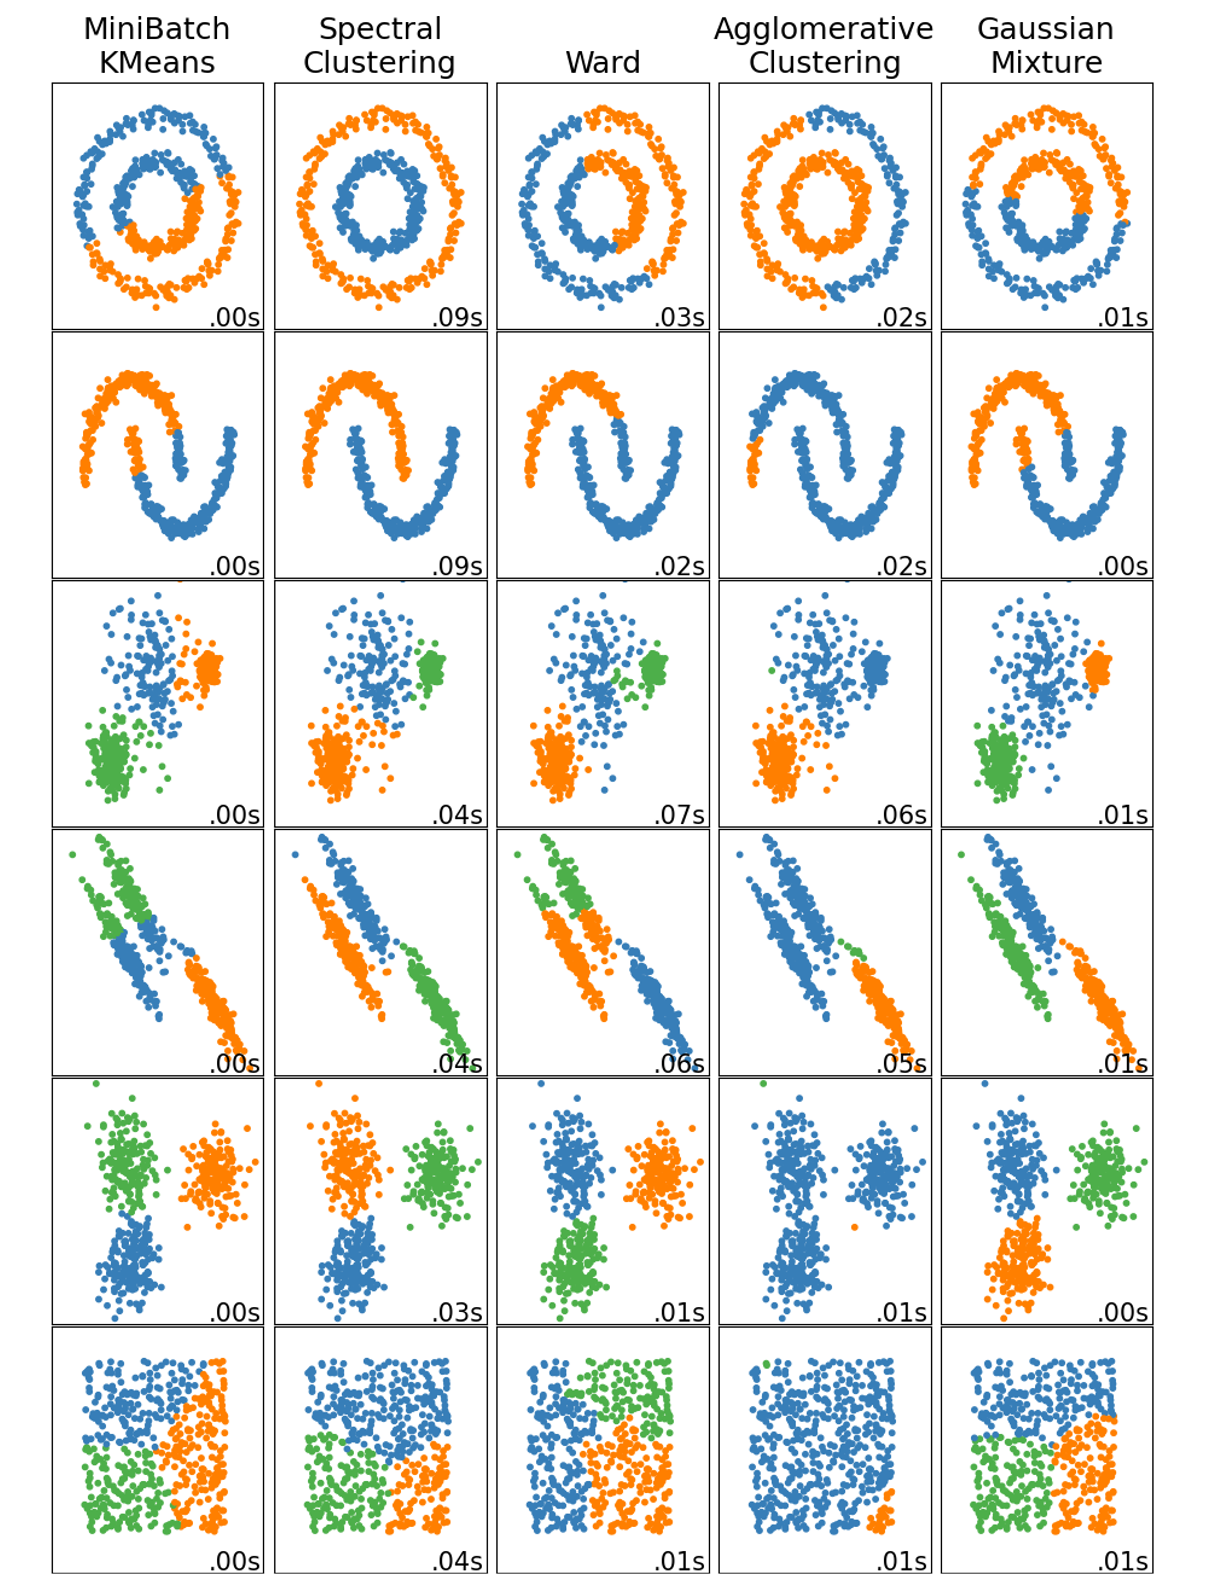
\includegraphics[width=0.8\textwidth,height=0.5\textheight,keepaspectratio]{Sections/Lit_review/Resources/clustering_scikit.png}
    \caption{How K-means (MiniBatch version), Spectral Clustering, Wards, Agglomerative Clustering, and Gaussian Mixture Models behave with different types of 2D datasets. Running times shown on the bottom right corner, all algorithms having comparable running times, with K-means being the fastest. Image adapted from \cite{Scikit-learn_undated-ax}}
    \label{fig:lit:clustering_types}
\end{figure}
\FloatBarrier

One of the most popular methods (and the simplest) is K-means clustering, which attempts to find patterns in the data by grouping data points by distance. There are variations of the algorithm where datasets are split into multiple batches to improve performance (see \textit{MiniBatch Kmeans} from \cref{fig:clustering_types}); or Fuzzy K-means that output the cluster membership of each data point. This means that apart from the cluster labelling, there is additional information about how close each point is to a cluster\footnote{For example, if there are 3 clusters, a data point might be 90\% in cluster 1, 6\% in cluster 2, and 4\% in cluster 3.}. From the below K-means pseudocode\footnote{Pseudocode is an accessible method to describe an algorithm.} (\cref{code:k-means}), a few things are worth emphasizing:

\begin{itemize}
  \item The number of centroids (K) is defined by the user.
  \item The distance between two points can be of different types; the Euclidean is common, but for higher dimensions, cosine is more suitable.
  \item Even though the centroids are randomly initialised, new values are computed at each step by averaging the distance of the points in that cluster to the old centroid.
  \item The algorithm converges when the centroids don't significantly change.
\end{itemize}

\begin{lstlisting}[caption={K-means pseudocode}, label={code:k-means}]
  Initialise the centroids at random positions
  while not converged 
    For each data point
      Compute the distance to all the centroids
      The closest represents the cluster to which the data point belongs
    Update the centroids based on the mean distance of each cluster
\end{lstlisting} 

Agglomerative clustering is a type of hierarchical clustering that starts by considering each data point as its cluster, then computes higher up groups based on the given linkage method. These algorithms (pseudocode in \cref{code:agg_clustering}) build hierarchical trees and can be seen visually in dendrogram figures, which are useful in visualising the clustering evolution. Both K-means and Agglomerative Clustering can use different types of distances, but the latter does not require setting the number of centroids; however, the dendrogram has to be chosen as well as the type of linkange method. This setting configures how the datapoint grouping is performed and the Scikit-learn supports the following\footnote{There is a nice visualisation for each of these hierarchical clustering in this \href{https://towardsdatascience.com/machine-learning-algorithms-part-12-hierarchical-agglomerative-clustering-example-in-python-1e18e0075019}{Medium post}}:
\begin{itemize}
  \item \textbf{Average} - Grouping is done by the average distance between cluster points.
  \item \textbf{Ward} - Merging clusters by the sum of squared distances. This linkage minimises the variance and is similar to K-means.
  \item \textbf{Single} - The distance between two groups is given by the two closest points. This considers merging clusters that have the closest points.
  \item \textbf{Complete} - The opposite to Single linkage, the distance between the two groups is given by the farthest points. This method looks at the outer layer points and may provide a more accurate grouping.
\end{itemize}

\begin{lstlisting}[caption={Agglomerative hierarchical clustering pseudocode}, label={code:agg_clustering}]
  To each data point assign a cluster number
  while more than one cluster
    Group the closest datapoints together 
    Smaller clusters morph together into larger ones
\end{lstlisting} 

Gaussian Mixture Models (GMM) are probabilistic models that assume all data points are generated from a mixture of a finite number of Gaussian distributions with unknown parameters. GMMs accommodate asymmetric clusters compared to K-means which assumes clusters are similar size. Another applied clustering algorithm in the project, Spectral Clustering, transforms the clustering problem into a graph-partitioning problem. It begins by constructing an affinity matrix based on the pairwise similarity of points. It then uses linear algebra to project the data into a latent space from which the clusters are identified using methods like K-means.

The clustering algorithms presented so far are used throughout the project, initially to establish a referential point independent of the methods used in other MIBC subtyping work \cite{Robertson2017-mg, Marzouka2018-ge, Kamoun2020-tj}. Then, the clustering models were used to stratify the output of the network approach. To measure the performance of these algorithms, the below metrics were used.


\subsubsection*{Clustering metrics} \label{s:lit:clustering_metrics}

One of the challenges in clustering is to measure the performance of grouping as there is no labelling or prior information on how the grouping should look like. This project uses the canonical metrics which are supported by Scikit-learn\cite{Pedregosa2011-ts,Scikit-learn_undated-ax}. These are:
\begin{itemize}
  \item \textbf{Silhouette Coefficient} - higher the better. A higher Silhouette Coefficient score relates to a model with better-defined clusters. This is the preferred method in project for reasons highlighted in \ref{} and it is been used by the MIBC consensus \citet{Kamoun2020-tj} to asses the cluster separation.
  % It can use different distances and the score is calculated per sample as it follows:
  % \begin{itemize}
  %   \item The mean distance between a sample and all other points in a class.
  %   \item The mean distance between a sample and all other points in the next nearest cluster.
  %   \item The total score for the dataset is the mean of the above two points.
  % \end{itemize}
  \item \textbf{Calinski-Harabasz Index} - higher the better. A higher Calinski-Harabasz score relates to a model with better-defined clusters.  The score is the index is the ratio of the sum of between-clusters dispersion and of inter-cluster dispersion for all clusters (where dispersion is defined as the sum of distances squared).
  \item \textbf{Davies-Bouldin Index} - lower the better. A lower Davies-Bouldin index relates to a model with better separation between the clusters. The index is the average ‘similarity’ between clusters, where the similarity is a measure that compares the distance between clusters with the size of the clusters themselves.
\end{itemize}


In addition to the above metrics, there is a popular heuristic procedure, the Elbow method, which aids in choosing the right number of clusters. In \cref{fig:elbow_method} the y-axis is represented by the distance of the points from their centroids, while the x-axis is the number of clusters. It can be seen that there is a point of inflexion when the number of clusters is set to five and that is considered to be the optimal number of clusters.

\begin{figure}[!htb]
  \centering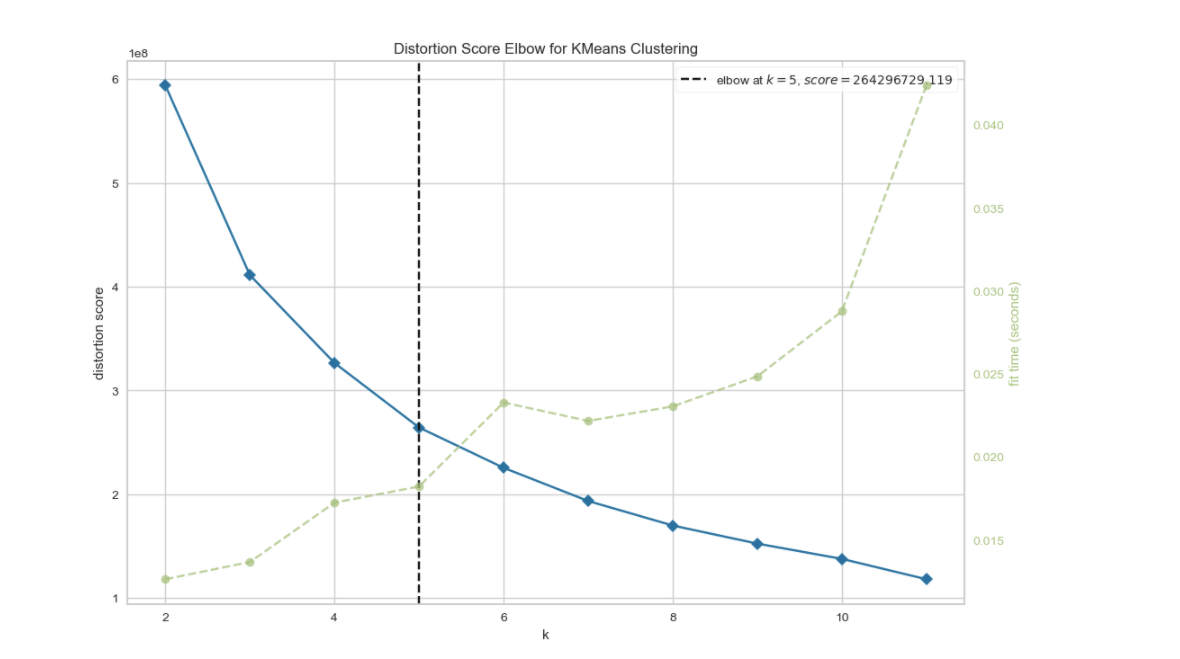
\includegraphics[width=0.7\textwidth,height=0.5\textheight,keepaspectratio]{Images/Clustering/elbow_method.png}
    \caption{Example of the elbow method, where 5 clusters are the optimal number of clusters. This has been applied on unpublished data of Benign Uropathies from Jack Birch Unit. The green line is the computational time. }
    \label{fig:elbow_method}
\end{figure}
\FloatBarrier


\subsubsection{Dimension reduction} \label{s:lit:dim_red}

In contrast to many computationally- or physics-focused data analysis problems, biologically derived datasets are characterised by a high number of features (dimension) and a small number of samples. Thus, it is often essential to use dimension reduction, \acrfull{pca} is the standard method that works by projecting the higher dimension to the specified lower dimension. For example, a principal component of a genomic dataset might be linked to biological sex, as it influences many features of a biological system.

However, this does not accommodate well with non-linear patterns for which UMAP (Uniform Manifold Approximation and Projection) and t-SNE (t Distributed Stochastic Neighbour Embedding) are used. Both are stochastic and non-linear dimension reduction techniques widely used in bioinformatics. UMAP is gaining popularity as it's been more stable in representing both within and between cluster sample relatedness. While, the method are good at reducing the data, their visualisation is misleading, as the proximity of points and clusters do not represent the 'closeness' of the data. Thus, when applying the two, the researcher needs to apply the clustering before the UMAP/t-SNE are applied, and then used the two for visualisation.

Another dimension reduction technique is \acrfull{nmf} which operates on the same principles as PCA which is by finding a matrix of a lower rank with the minimum information loss. This means that the features present in the data are preserved better when reduced to lower dimensions while the ones that do not contribute to the data resolution are discarded. In addition, NMF conserves the non-linear aspects of the data and a Bayesian version was used in the \acrfull{tcga} classification by \citet{Robertson2017-mg}. NMF also were used in the works of propagating (mutation) data into the networks by \citet{Yang2016-dm, Cai2008-fv} and covered in \cref{s:lit:net_prop}.

PCA is extensively used in this project, initially to reduce the data in \ref{} (subtypes section), and subsequently as a proxy metric to gauge the amount of variance contained in a subset of genes. This approach has been particularly useful in the network chapters, where multiple graphs are generated, each outputting a different subset of genes for clustering the MIBC.


\subsubsection{Graphs} \label{s:lit:graph_overview}

Genes impact each other, and there is a relationship between different subsets of genes that give rise to pathways, which are necessary for various functions in the tissue. The key aspect in genetics is the interdependence between elements. Traditional clustering analysis such as hierarchical clustering does not take these relationships into account, partly because they are not known, and also because the computational models do not have that layer of information built-in. Co-expressed networks are one way to model such connections by computing the pairwise correlation of gene expression to determine the strength of connections; the research done in this area is presented in \cref{s:lit:co_net}. The gene relationships can be represented in a graph or network, where a node (or vertex) represents a gene and an edge represents the connection between them; see \cref{fig:graphs_basic}.

\begin{figure}[!htb]
  \centering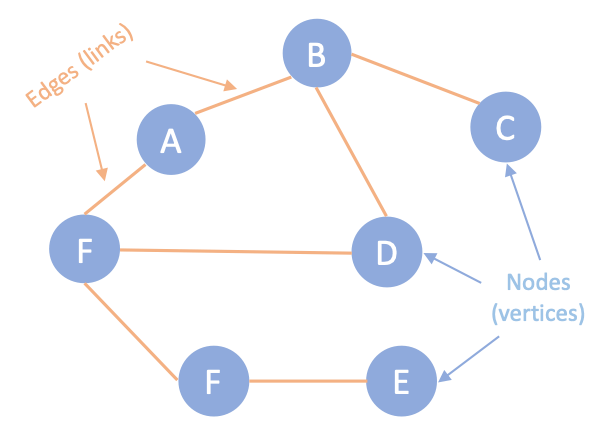
\includegraphics[width=0.5\textwidth,height=0.5\textheight,keepaspectratio]{Sections/Lit_review/Resources/basic_graphs.png}
    \caption{Basic graphs illustrating gene interactions.}
    \label{fig:graphs_basic}
\end{figure}

To establish how genes are linked in a network and interact, the edges are assigned values that reinforce the links between nodes (genes), and this data can be tabulated and processed by various graph algorithms. The edges weights represent an opportunity to model the different data types available in the omics. The work on integrating multiple data type is covered in \cref{s:lit:net_data_int}.

One aspect of graph analysis is to identify influential nodes, which in biology could involve finding genes that have a significant impact on the network, such as Transcription Factors (TFs). Another aspect of network theory involves examining nodes (i.e., genes) that can be grouped together; this is explored extensively in \cref{s:lit:comm_detect}. Graphs are intuitive for understanding and visualising, thus making them an effective tool for navigating high-dimensional data.

The challenge with graphs is that they are less developed and can be computationally taxing. For example, community detection is a hot topic because there is no established method for identifying groups of nodes, and some popular methods can find patterns in noise. These issues are discussed at length in \cref{s:lit:comm_detect}.

% Keep this section simple. It links to parts of your project you haven't discussed yet and so becomes a bit unclear. Effectively you want to state that genes can be linked in a network and that many biological approaches allow measurements of genes. This means you can infer relationships, see how relationships change in disease/perturbation and assess how distinct, but linked-in-the-network perturbations can lead to a common result/phenotype/observation


\subsubsection{Evolutionary Algorithms} \label{s:lit:ea_overview}

% In the previous section described how graphs are used to analyse the gene interactions and a similar approach but the different algorithm is \acrfull{cgp}. This is part of the \acrfull{ea} family which draws inspiration from the Darwinian evolution.

\acrlong{ea} are a type of \acrshort{ml} that draws inspiration from Darwinian evolution. By incorporating random changes in the algorithm, EA can be used for optimisation or search problems. Thus, EAs are suitable for doing a wide search of the solution space\footnote{Imagine the solution space as space of the total possible solutions for a problem.} which means that they might find an unusual solution and escape the local minimum. A useful analogy here is to think as one climbing a mountain (search space), the goal (optimal solution) is to reach the highest peak but along the way, there are other peaks (local minimum) but smaller (less optimal) than the highest peak (optimal solution). The process (algorithm) in reaching the desired peak is incremental and it requires choosing the right path to reach the global top. Usually, an algorithm has difficulties in differentiated between the highest peaks and the smaller ones, but due to the high variation characteristic of EA, these methods perform well in such problems.


However, these algorithms have a high computational cost and do not usually scale well, therefore are applied to relatively small problems (i.e. number of features). The corollary is that EAs are easier to understand compared to the  \acrfull{dl} (explored in \cref{s:lit:dl_genomics}) and are classified as a 'white-box' approach. In \cref{s:lit:mutations} is presented the MDPFinder (\citet{Zhao2012-wj}) model where \acrfull{ga}, a simpler version of EAs, are applied to process both Gene Expression and mutations.

% would split the sentence here. You could then link to your next point, perhaps: "...from Darwinian evolution. By incorporating random changes in the parameters of a model, or set of models, EA can be used for optimisation..." Something like this makes it clearer why the Darwinian principles are important

As EA resembles the evolutionary process there is also some shared terminology, an individual in the EA context represents a potential solution and a population is a collection of potential solutions. \Cref{fig:ea_basic} describes the algorithmic flow of the evolutionary approach which starts with the initialisation stage, where the individuals are given (usually) random values, followed by the second stage where the fitness of the individuals is measured; i.e. how suitable they are for the problem. If the problem is not solved, then select only the fittest individuals which are then mutated/crossover, introducing variation to the new population. Like in biology, this last step, gives EA a large variety of individuals. This set of steps is run until an individual fits the solution/problem. It is worth mentioning, that the mutation rate, crossover and how the individual is selected, are preset parameters. 

\begin{figure}[!htb]
  \centering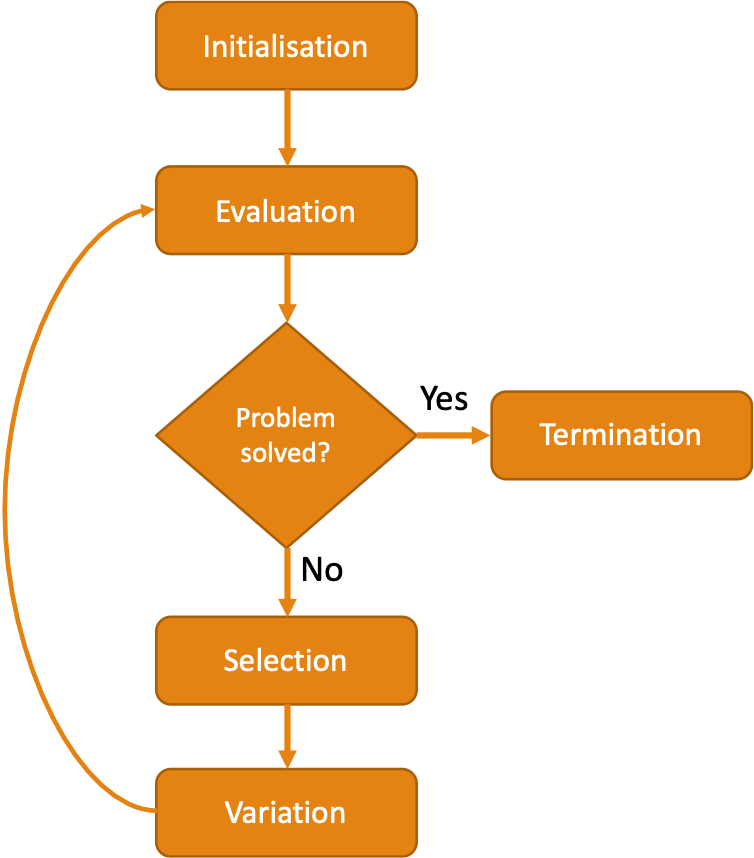
\includegraphics[width=0.4\textwidth,height=0.4\textheight,keepaspectratio]{Images/Resources/EA_basic.png}
    \caption{Evolutionary Algorithms algorithm.}
    \label{fig:ea_basic}
\end{figure}
\FloatBarrier


Defining the fitness function as well as encoding the data for the EA algorithm is one of the challenges when developing EA as it is problem specific. Biological evolution is a process that takes time and many iterations, the in-silico adaptation share that and it is the reason for not scaling well or as it has a high computational cost.

The MDPFinder model presented in \cref{s:lit:mutations} used a variation of EA, called \acrfull{ga} which is a simpler version of the EA family where individuals resemble the chromosome. \acrfull{cgp} is another EA algorithm which it's used to process graph representation and it overcomes some of the limitations of the simpler EA methods. 


\subsubsection{Artificial Neural Networks} \label{s:lit:ann_overview}

Artificial Neural Networks (ANN) are the ML strand that have been pushing the AI breakthroughs in the past 20 years. The inspiration comes from how the brain draws the information from the external stimuli, stores it in memory and retrieve it. Despite being many unknowns to the brain, the main components that are involved in the learning process are the neurons and the synapses between them\footnote{The neurons and synapses are the main components, but there may be others like dendrites which can also be computational units as seen later in the section.}. The simplest learning rule was introduced by Donald Hebb which states "Neurons that fire together, wire together"\cite{Hebb_Donald1949-nn}. This means that a neuron that fire or its concurrently activated with another one (or in a given time window) the two form a stronger connection. The opposite is true, the synapse is weaken, when two neurons that do not get activated in the same time window.

\begin{figure}[!htb]
  \centering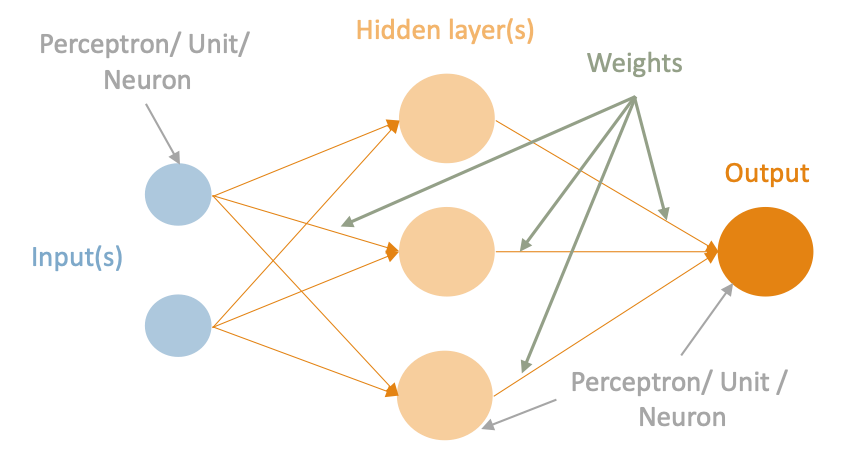
\includegraphics[width=0.7\textwidth,height=0.7\textheight,keepaspectratio]{Images/ANN/Basic_ANN.png}
    \caption{A Simple ANN architecture. }
    \label{fig:ann_basic}
\end{figure}
\FloatBarrier

\Cref{fig:ann_basic} it's a simple, single-layer, feed-forward Neural Network where a layer represents a collection of units that usually have the same activation function. In the case of \acrfull{dnn}, the ANN is constructed by many such layers with a large number of units. The neurons are the computational component, each having an activation function that 'tells' the unit when to activate and send a signal across the synapse. The connections between the units are assigned a weight that gives the strength of the synapses. The information is stored in the connections between the units, and it follows Donald Hebb's learning rule stated earlier. Therefore, the central goal of ANN is to find the specific configuration of weight values that gives the desired output. Previously, we mentioned different types of learning, in the supervised case, there is an algorithm that has been the engine of the connectionist approach, called back-propagation. As the name suggests, this method propagates the input's error from the output layer back, this information is used then to compute new values for the network's weights; this is called stochastic gradient descent.

\paragraph*{Autoencoders} \label{s:lit:autoencod_overview}

Autoencoders are a particular type of Deep Neural Networks and \cref{fig:autoencoders} represents a diagram a simple Autoencoder architecture in which it can be seen that there are 3 main components. The input layer to which the data is fed, for more complex models it has additional hidden layers and with the input, the two layers are known together as the encoder stage. The bottleneck part is where the data is compressed into a lower dimension. Next, a mirror to the encoder, the decoder, is dealing with reconstructing the outputs of the bottleneck into original data; hence, the name. This part of autoencoders is an advantage over the PCA as the original data can be reconstructed from the lower dimension. A derivative of Neural Networks, autoencoders are more suitable to find non-linear patterns in the data as whereas PCA finds only linear patterns. With all these advantages as dimension reduction techniques is not a surprise that there has been some work on applying Autoencoders to genomics (explored further in \cref{s:lit:autoencoders}).

\begin{figure}[!htb]
  \centering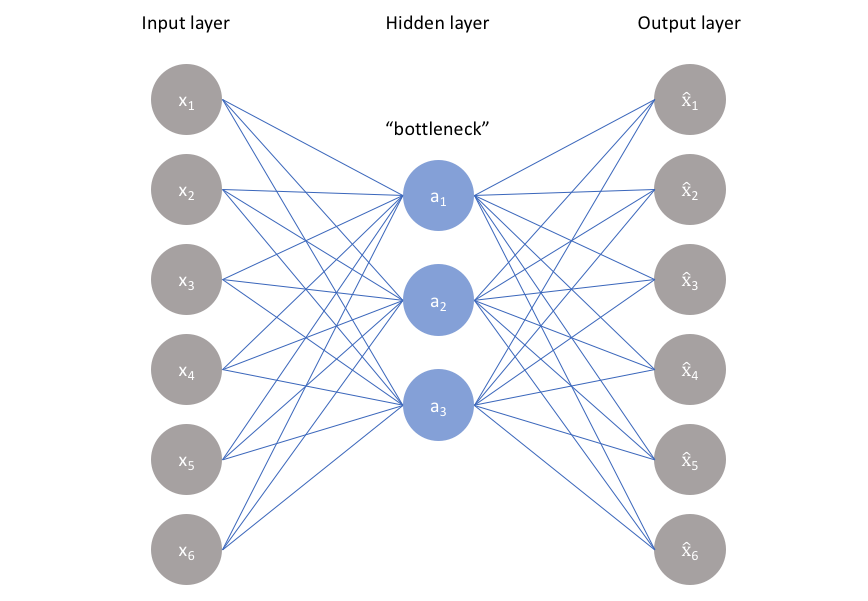
\includegraphics[width=0.8\textwidth,height=0.5\textheight,keepaspectratio]{Images/Autoencoders/simple_autoencoders.png}
    \caption{Simple architecture of autoencoders, from \cite{Jordan2018-bc}}
    \label{fig:autoencoders}
\end{figure}
\FloatBarrier

Autoencoders are the most successful \acrshort{dnn} approaches to genomics problems where they have been used as a dimension reduction technique to solve the dimension curse of genetic data, where few samples are available with a large number of features (genes). This means, that they are not replacing the clustering models but techniques like \acrfull{pca} or \acrfull{nmf}, and will be used in conjunction with clustering techniques.


\subsubsection{Summary} \label{s:lit:choosing_ml}

\Cref{s:lit:ea_overview} covered the basics of the evolutionary approach, and in both \ref{s:lit:ann_overview} and \ref{s:lit:autoencod_overview} sections, the connectionists' view of ML was presented. These two methodologies address different types of problems: EAs are more suited for search problems, while ANNs excel in classification tasks. ANNs operate by optimising the configuration of weights and network topology, which can be seen as a search/optimisation challenge to find the right network configuration. 

Consequently, there has been significant research into combining these two approaches in what is termed Neuroevolution. This approach has been employed to process mutation data, as discussed in \cref{s:lit:mutations}. In these computational methods, EAs are used to establish the optimal initial configuration of the ANN, which is then used for training. Starting from a state other than random helps the ANN to circumvent the local minimum problem and enhance classification performance. Additionally, EAs are employed to determine the best network topology, including the number of layers, units, and their connections.

From an engineering perspective, the problem studied in this project is characterised by a large number of features and a small number of samples. It is an unsupervised learning type problem, which needs to determined the groups in an unlabelled data. There are multiple levels of information available for each gene which includes gene expression, mutations and epigenetic data. Therefore, it is important to choose a computational method that satisfy the project's aims and objectives. The next section aims to review the work done across the genomics field by examining various approaches depending on the datasets used.
